% !TEX program = xelatex
\documentclass[notheorems,aspectratio=169]{beamer}
\usepackage{ctex,fontspec,xeCJK}
\IfFontExistsTF{Noto Serif CJK JP}{\setCJKmainfont{Noto Serif CJK JP}\setCJKsansfont{Noto Sans CJK JP}}{}
\usepackage{amsmath,amssymb,bm,booktabs,array,multicol}
\usepackage{tikz}
\usetikzlibrary{arrows.meta,calc,positioning,shapes.geometric,decorations.pathmorphing,patterns}
\usetheme{Madrid}
\usefonttheme[onlymath]{serif}
\beamertemplatenavigationsymbolsempty
\let\Tiny\tiny

\definecolor{ChinaRed}{RGB}{196,30,58}
\definecolor{JapanBlue}{RGB}{0,82,155}
\definecolor{SoftBlue}{RGB}{231,241,249}
\definecolor{SoftRed}{RGB}{252,235,239}
\definecolor{GraphGray}{RGB}{94,103,112}
\definecolor{ChemGreen}{RGB}{29,132,96}
\definecolor{SoftGreen}{RGB}{232,246,240}
\definecolor{Gold}{RGB}{215,153,33}
\definecolor{Purple}{RGB}{116,78,160}
\setbeamercolor{structure}{fg=JapanBlue}
\setbeamercolor{alerted text}{fg=ChinaRed}
\setbeamercolor{block title alerted}{bg=ChinaRed,fg=white}
\setbeamercolor{block body alerted}{bg=SoftRed}
\setbeamercolor{block title}{bg=JapanBlue,fg=white}
\setbeamercolor{block body}{bg=SoftBlue}
\setbeamercolor{block title example}{bg=ChemGreen,fg=white}
\setbeamercolor{block body example}{bg=SoftGreen}
\setbeamertemplate{itemize item}{\color{JapanBlue}$\blacktriangleright$}
\setbeamertemplate{itemize subitem}{\color{ChinaRed}$\bullet$}
\newcommand{\jp}[1]{\textbf{\color{JapanBlue}#1}}
\newcommand{\key}[1]{\textbf{\color{ChinaRed}#1}}
\newcommand{\en}[1]{\textcolor{GraphGray}{\scriptsize(#1)}}
\newcommand{\ans}[1]{\textcolor{ChemGreen}{\textbf{答：}#1}}
\newcommand{\electron}[2]{\fill[ChinaRed] (#1,#2) circle (2.2pt);}
\newcommand{\atom}[3]{\node[circle,draw=#3,fill=#3!12,minimum size=9mm,font=\bfseries] at (#1) {#2};}
\setbeamercolor{question card}{fg=black,bg=SoftRed}
\setbeamercolor{answer card}{fg=black,bg=SoftGreen}
\newcommand{\questioncard}[1]{%
  \begin{columns}[c,onlytextwidth]
    \column{.10\textwidth}\centering
\begin{tikzpicture}\node[circle,fill=ChinaRed,text=white,font=\Large\bfseries,minimum size=10mm]{Q};\end{tikzpicture}
    \column{.87\textwidth}\begin{beamercolorbox}[rounded=true,shadow=true,sep=1.1ex]{question card}#1\end{beamercolorbox}
  \end{columns}}
\newcommand{\answercard}[1]{%
  \begin{columns}[c,onlytextwidth]
    \column{.10\textwidth}\centering
\begin{tikzpicture}\node[circle,fill=ChemGreen,text=white,font=\Large\bfseries,minimum size=10mm]{A};\end{tikzpicture}
    \column{.87\textwidth}\begin{beamercolorbox}[rounded=true,shadow=true,sep=1.1ex]{answer card}#1\end{beamercolorbox}
  \end{columns}}
\newcommand{\reasonflow}[3]{%
  \begin{center}\begin{tikzpicture}[>=Latex,node distance=5mm,flow/.style={draw=JapanBlue,fill=SoftBlue,rounded corners=2mm,minimum width=30mm,minimum height=9mm,align=center,font=\small\bfseries}]
    \node[flow] (a) {#1};\node[flow,right=of a] (b) {#2};\node[flow,right=of b] (c) {#3};
    \draw[->,very thick,ChinaRed] (a)--(b);\draw[->,very thick,ChinaRed] (b)--(c);
  \end{tikzpicture}\end{center}}

\title[EJU Chemistry]{化学2}
\subtitle{電子配置・元素の周期律・化学結合と結晶}
\author[Sirui Liu]{Sirui Liu}
\date{2026年7月}

\begin{document}
\begin{frame}\titlepage\end{frame}

\begin{frame}{本時の目標}
\begin{columns}[T,onlytextwidth]
\column{.48\textwidth}
\begin{block}{電子と周期表}
\begin{itemize}
  \item 電子配置を殻・軌道で表す
  \item 族・周期と価電子を結びつける
  \item 原子半径・イオン化エネルギーの傾向を説明する
\end{itemize}
\end{block}
\column{.48\textwidth}
\begin{exampleblock}{結合と結晶}
\begin{itemize}
  \item イオン結合と共有結合を区別する
  \item 分子間力から沸点を比較する
  \item 結晶の種類から性質を予測する
\end{itemize}
\end{exampleblock}
\end{columns}
\begin{alertblock}{解题主线}
\centering 原子番号 $\rightarrow$ 電子配置 $\rightarrow$ 価電子 $\rightarrow$ 結合 $\rightarrow$ 物質の性質
\end{alertblock}
\end{frame}

\begin{frame}{目次}\tableofcontents\end{frame}

% ================================================================
\section{電子配置}

\begin{frame}{原子核と電子殻}
\begin{columns}[c,onlytextwidth]
\column{.45\textwidth}
\centering
\begin{tikzpicture}[scale=.88]
  \fill[Gold] (0,0) circle (8mm);
  \node[font=\bfseries] at (0,0){核};
  \draw[JapanBlue,thick] (0,0) circle (1.25);
  \draw[ChemGreen,thick] (0,0) circle (2.15);
  \draw[Purple,thick] (0,0) circle (3.0);
  \foreach \a in {45,225}{\fill[ChinaRed] (\a:1.25) circle (2.5pt);}
  \foreach \a in {0,45,...,315}{\fill[ChinaRed] (\a:2.15) circle (2.5pt);}
  \foreach \a in {0,60}{\fill[ChinaRed] (\a:3.0) circle (2.5pt);}
  \node[JapanBlue] at (1.05,1.05){K};
  \node[ChemGreen] at (1.75,1.75){L};
  \node[Purple] at (2.42,2.42){M};
\end{tikzpicture}
\column{.51\textwidth}
\begin{block}{電子殻（电子层）}
电子只能取离散能量。离原子核越远，一般能量越高。
\end{block}
\begin{itemize}
  \item K殻：$n=1$
  \item L殻：$n=2$
  \item M殻：$n=3$
  \item 最外殻の電子 $\Rightarrow$ \jp{最外殻電子}
\end{itemize}
\end{columns}
\end{frame}

\begin{frame}{各電子殻に入る最大電子数}
\begin{columns}[T,onlytextwidth]
\column{.46\textwidth}
\begin{block}{最大収容数}
主量子数を $n$ とすると
\[
\boxed{N_{\max}=2n^2}
\]
\end{block}
\begin{center}
\begin{tabular}{c@{\qquad}c@{\qquad}c}\toprule
殻 & $n$ & 最大数\\\midrule
K & 1 & 2\\
L & 2 & 8\\
M & 3 & 18\\
N & 4 & 32\\\bottomrule
\end{tabular}
\end{center}
\column{.49\textwidth}
\begin{alertblock}{注意}
“最大可容纳数”和“基态原子中按顺序填入的数”不是同一个问题。K、L殻填满后，电子会先进入能量较低的轨道。
\end{alertblock}
\begin{exampleblock}{例}
Ca（原子番号20）の殻表示は
\[
\boxed{2,\ 8,\ 8,\ 2}
\]
M殻并未达到最大18，就已开始进入N殻。
\end{exampleblock}
\end{columns}
\end{frame}

\begin{frame}{電子配置の二つの表し方}
\begin{columns}[T,onlytextwidth]
\column{.47\textwidth}
\begin{block}{殻表示}
Na（原子番号11）
\[
\boxed{2,\ 8,\ 1}
\]
适合快速判断周期、最外层电子数和常见离子。
\end{block}
\column{.49\textwidth}
\begin{exampleblock}{軌道表示 \en{orbital notation}}
\[
\boxed{1s^2\,2s^2\,2p^6\,3s^1}
\]
上标表示该轨道所含电子数。
\end{exampleblock}
\end{columns}
\vfill
\centering
\begin{tikzpicture}[>=Latex,node distance=9mm]
\node[draw,rounded corners,fill=SoftBlue,minimum width=28mm,minimum height=10mm] (z) {原子番号 11};
\node[draw,rounded corners,fill=SoftGreen,right=of z,minimum width=32mm,minimum height=10mm] (e) {電子数 11};
\node[draw,rounded corners,fill=SoftRed,right=of e,minimum width=38mm,minimum height=10mm] (c) {電子配置を作る};
\draw[->,very thick,JapanBlue] (z)--(e);\draw[->,very thick,ChinaRed] (e)--(c);
\end{tikzpicture}
\end{frame}

\begin{frame}{軌道：電子が入る「部屋」}
\small
\begin{columns}[c,onlytextwidth]
\column{.52\textwidth}
\begin{center}
\begin{tabular}{c c c c}\toprule
副殻 & 軌道数 & 最大電子数 & 形のイメージ\\\midrule
$s$ & 1 & 2 & 球形\\
$p$ & 3 & 6 & 互いに直交\\
$d$ & 5 & 10 & より複雑\\
$f$ & 7 & 14 & より複雑\\\bottomrule
\end{tabular}
\end{center}
\column{.44\textwidth}
\centering
\begin{tikzpicture}[scale=.9]
  \shade[ball color=JapanBlue!45,opacity=.65] (-1.7,1.1) circle (.72);
  \node at (-1.7,-.05){$s$ 軌道};
  \shade[ball color=ChinaRed!55,opacity=.7] (1.2,1.65) ellipse (.52 and .9);
  \shade[ball color=ChinaRed!55,opacity=.7] (1.2,.55) ellipse (.52 and .9);
  \fill[Gold] (1.2,1.1) circle (2pt);
  \node at (1.2,-.05){$p$ 軌道の一つ};
\end{tikzpicture}
\end{columns}
\begin{alertblock}{一つの軌道には最大2個}
两电子进入同一轨道时，自旋方向相反：$\boxed{\uparrow\downarrow}$。
\end{alertblock}
\end{frame}

\begin{frame}{電子を入れる三つの規則}
\begin{enumerate}
  \item \jp{構築原理}：能量低的轨道优先填入。
  \item \jp{パウリの排他原理}：一个轨道最多2个电子，且自旋相反。
  \item \jp{フントの規則}：同能量轨道先各自单独填入，再成对。
\end{enumerate}
\vfill
\centering
\begin{tikzpicture}[x=1.25cm,y=.9cm]
\foreach \x in {0,1,2}{\draw[thick] (\x,0) rectangle ++(.8,.55);}
\draw[->,very thick,JapanBlue] (.2,.08)--(.2,.47);
\draw[->,very thick,JapanBlue] (1.2,.08)--(1.2,.47);
\draw[->,very thick,JapanBlue] (2.2,.08)--(2.2,.47);
\node at (1.4,-.45){$p^3$：\key{先分别占据三个轨道}};
\begin{scope}[xshift=6cm]
\foreach \x in {0,1,2}{\draw[thick] (\x,0) rectangle ++(.8,.55);}
\draw[->,very thick,GraphGray] (.2,.08)--(.2,.47);
\draw[<-,very thick,GraphGray] (.58,.08)--(.58,.47);
\draw[->,very thick,GraphGray] (1.2,.08)--(1.2,.47);
\node[GraphGray] at (1.4,-.45){错误：过早配对};
\end{scope}
\end{tikzpicture}
\end{frame}

\begin{frame}{軌道のエネルギー順序}
\begin{columns}[c,onlytextwidth]
\column{.58\textwidth}
\centering
\begin{tikzpicture}[x=1.05cm,y=.72cm,>=Latex]
\foreach \name/\x/\y in {1s/0/0,2s/0/1,2p/1/1,3s/0/2,3p/1/2,3d/2/2,4s/0/3,4p/1/3,4d/2/3,4f/3/3}{
  \node[draw,rounded corners,fill=SoftBlue,minimum width=9mm] at (\x,\y){$\name$};}
\draw[->,very thick,ChinaRed] (-.45,-.45)--(3.6,3.65) node[above]{能量升高};
\end{tikzpicture}
\column{.38\textwidth}
\begin{block}{常用填充顺序}
\[
\begin{aligned}
1s&\to2s\to2p\to3s\\
&\to3p\to4s\to3d\\
&\to4p\to\cdots
\end{aligned}
\]
\end{block}
\begin{alertblock}{EJU重点}
主族元素通常重点掌握到 Ca；过渡元素需注意 $4s$ 与 $3d$。
\end{alertblock}
\end{columns}
\end{frame}

\begin{frame}{価電子と最外殻電子}
\small
\begin{columns}[T,onlytextwidth]
\column{.48\textwidth}
\begin{block}{最外殻電子（最外层电子）}
主量子数最大的电子层中的电子。
\end{block}
\begin{exampleblock}{価電子（价电子）}
实际参与化学键、决定化学性质的电子。
\end{exampleblock}
\column{.48\textwidth}
\begin{center}
\begin{tabular}{c c c}\toprule
原子 & 電子配置 & 価電子\\\midrule
Na & $2,8,1$ & 1\\
Mg & $2,8,2$ & 2\\
Cl & $2,8,7$ & 7\\
Ar & $2,8,8$ & 0\\\bottomrule
\end{tabular}
\end{center}
\end{columns}
\begin{alertblock}{希ガス}
稀有气体最外层已稳定，一般把价电子数记作0，因此化学性质很不活泼。
\end{alertblock}
\end{frame}

\begin{frame}{イオンになると電子配置はどう変わるか}
\begin{columns}[c,onlytextwidth]
\column{.46\textwidth}
\begin{block}{陽イオン（阳离子）}
原子失去电子：
\[
\mathrm{Na}\ (2,8,1)\rightarrow \mathrm{Na^+}\ (2,8)+e^-
\]
\end{block}
\column{.50\textwidth}
\begin{alertblock}{陰イオン（阴离子）}
原子得到电子：
\[
\mathrm{Cl}+e^-\rightarrow \mathrm{Cl^-}
\]
\[
(2,8,7)\qquad\ \ (2,8,8)
\]
\end{alertblock}
\end{columns}
\vfill
\reasonflow{価電子を数える}{最少の授受を考える}{希ガス型へ近づく}
\end{frame}

\begin{frame}{例題1｜電子配置：問題}
\def\exq{次の原子について、殻による電子配置と価電子数を答えよ。\quad (1) O（原子番号8）\quad (2) Al（13）\quad (3) Ca（20）}
\only<1>{\vfill\questioncard{\exq}\vfill}
\only<2>{\questioncard{\exq}\vfill
\begin{center}\begin{tabular}{c c c}\toprule 原子 & 殻表示 & 価電子数\\\midrule O & $2,6$ & 6\\ Al & $2,8,3$ & 3\\ Ca & $2,8,8,2$ & 2\\\bottomrule\end{tabular}\end{center}
\answercard{中性原子的电子数等于原子番号；从K殻开始按低能量顺序填入。}}
\end{frame}

\begin{frame}{例題2｜イオン：問題}
\def\exq{Mg、O、Cl が安定な単原子イオンになるとき、イオン式と電子数を答えよ。原子番号は Mg=12、O=8、Cl=17 とする。}
\only<1>{\vfill\questioncard{\exq}\vfill}
\only<2>{\questioncard{\exq}\vfill
\reasonflow{原子の電子数}{失うか受け取るか}{イオンの電子数}
\answercard{$\mathrm{Mg^{2+}}$：10個、$\mathrm{O^{2-}}$：10個、$\mathrm{Cl^-}$：18個。电荷 $=\text{质子数}-\text{电子数}$。}}
\end{frame}

% ================================================================
\section{元素の周期律と周期表}

\begin{frame}{元素の周期律（元素周期律）}
\begin{block}{現代的な定義}
元素を\jp{原子番号}の順に並べると、元素の物理的・化学的性質が周期的に変化する。
\end{block}
\begin{columns}[c,onlytextwidth]
\column{.56\textwidth}
\centering
\begin{tikzpicture}[x=.78cm,>=Latex,node distance=7mm]
\foreach \t/\x/\c in {Li/0/JapanBlue,Be/1/JapanBlue,B/2/ChemGreen,C/3/ChemGreen,N/4/ChemGreen,O/5/ChinaRed,F/6/ChinaRed,Ne/7/Gold}{
\node[draw=\c,fill=\c!12,minimum size=7mm,font=\small\bfseries] (n\x) at (\x,0){\t};}
\draw[->,very thick,GraphGray] (-.5,-.75)--(7.5,-.75) node[midway,below]{原子番号};
\end{tikzpicture}
\column{.40\textwidth}
\begin{itemize}
  \item 最外殻電子数逐步变化
  \item 金属性逐渐减弱
  \item 周期末出现希ガス
  \item 下一周期重复类似规律
\end{itemize}
\end{columns}
\end{frame}

\begin{frame}{周期表の読み方：周期と族}
\centering
\begin{tikzpicture}[x=.58cm,y=.58cm,font=\scriptsize]
\foreach \g in {1,...,18}{\node[GraphGray] at (\g,7.45){\g};}
\foreach \p in {1,...,7}{\node[GraphGray] at (.2,{7-\p}){\p};}
\foreach \g in {1,...,18}{\foreach \p in {1,...,7}{\draw[GraphGray!40] (\g-.42,{7-\p-.35}) rectangle ++(.84,.7);}}
\fill[JapanBlue!20] (.58,5.65) rectangle (1.42,-.35);
\fill[ChinaRed!17] (16.58,5.65) rectangle (17.42,-.35);
\fill[Gold!25] (17.58,6.65) rectangle (18.42,-.35);
\fill[SoftGreen] (1.58,0.65) rectangle (18.42,-.35);
\node[font=\bfseries] at (1,6){H};\node[font=\bfseries] at (18,6){He};
\node[JapanBlue,font=\bfseries] at (1,3){1族};
\node[ChinaRed,font=\bfseries,rotate=90] at (17,2.2){17族：ハロゲン};
\node[Gold!60!black,font=\bfseries,rotate=90] at (18,2.2){18族：希ガス};
\draw[->,very thick,JapanBlue] (3,7.8)--(9,7.8) node[right]{族：縦列};
\draw[->,very thick,ChinaRed] (-.5,5.5)--(-.5,1.5) node[below]{周期：横行};
\end{tikzpicture}
\begin{alertblock}{基本対応}
\centering 周期番号 $=$ 電子殻の数（主族）\qquad 族から価電子数を判断できる
\end{alertblock}
\end{frame}

\begin{frame}{典型元素の族と価電子}
\small
\centering
\begin{tabular}{c c c c c c}\toprule
族 & 1 & 2 & 16 & 17 & 18\\\midrule
価電子数 & 1 & 2 & 6 & 7 & 0\\
代表元素 & Li, Na, K & Mg, Ca & O, S & F, Cl, Br & He, Ne, Ar\\
常见离子 & $+1$ & $+2$ & $-2$ & $-1$ & 不形成\\\bottomrule
\end{tabular}
\vfill
\begin{columns}[T,onlytextwidth]
\column{.31\textwidth}\begin{block}{アルカリ金属}1族（H除外）。水と反应しやすい。下方越活泼。\end{block}
\column{.31\textwidth}\begin{alertblock}{ハロゲン}17族。二原子分子，易得到1电子。\end{alertblock}
\column{.31\textwidth}\begin{exampleblock}{希ガス}18族。闭壳层，化学性质稳定。\end{exampleblock}
\end{columns}
\end{frame}

\newcommand{\ptcell}[4]{%
  \path[draw=white,line width=.35pt,rounded corners=.5pt,fill=#4]
    ({#2-1},{1-#3}) rectangle ++(.92,.82);
  \node[font=\fontsize{4.5}{5}\selectfont\bfseries,text=black!78]
    at ({#2-.54},{1.41-#3}) {#1};}

\begin{frame}{金属元素・非金属元素・半金属}
\begin{columns}[c,onlytextwidth]
\column{.54\textwidth}
\centering
\begin{tikzpicture}[x=.36cm,y=.50cm]
% 第1周期
\ptcell{H}{1}{1}{SoftGreen}
\ptcell{He}{18}{1}{SoftGreen}
% 第2周期
\ptcell{Li}{1}{2}{JapanBlue!28}\ptcell{Be}{2}{2}{JapanBlue!28}
\ptcell{B}{13}{2}{SoftRed}\ptcell{C}{14}{2}{SoftGreen}
\ptcell{N}{15}{2}{SoftGreen}\ptcell{O}{16}{2}{SoftGreen}
\ptcell{F}{17}{2}{SoftGreen}\ptcell{Ne}{18}{2}{SoftGreen}
% 第3周期
\ptcell{Na}{1}{3}{JapanBlue!28}\ptcell{Mg}{2}{3}{JapanBlue!28}
\ptcell{Al}{13}{3}{JapanBlue!28}\ptcell{Si}{14}{3}{SoftRed}
\ptcell{P}{15}{3}{SoftGreen}\ptcell{S}{16}{3}{SoftGreen}
\ptcell{Cl}{17}{3}{SoftGreen}\ptcell{Ar}{18}{3}{SoftGreen}
% 第4周期
\ptcell{K}{1}{4}{JapanBlue!28}\ptcell{Ca}{2}{4}{JapanBlue!28}
\ptcell{Sc}{3}{4}{JapanBlue!28}\ptcell{Ti}{4}{4}{JapanBlue!28}
\ptcell{V}{5}{4}{JapanBlue!28}\ptcell{Cr}{6}{4}{JapanBlue!28}
\ptcell{Mn}{7}{4}{JapanBlue!28}\ptcell{Fe}{8}{4}{JapanBlue!28}
\ptcell{Co}{9}{4}{JapanBlue!28}\ptcell{Ni}{10}{4}{JapanBlue!28}
\ptcell{Cu}{11}{4}{JapanBlue!28}\ptcell{Zn}{12}{4}{JapanBlue!28}
\ptcell{Ga}{13}{4}{JapanBlue!28}\ptcell{Ge}{14}{4}{SoftRed}
\ptcell{As}{15}{4}{SoftRed}\ptcell{Se}{16}{4}{SoftGreen}
\ptcell{Br}{17}{4}{SoftGreen}\ptcell{Kr}{18}{4}{SoftGreen}
% 第5周期
\ptcell{Rb}{1}{5}{JapanBlue!28}\ptcell{Sr}{2}{5}{JapanBlue!28}
\ptcell{Y}{3}{5}{JapanBlue!28}\ptcell{Zr}{4}{5}{JapanBlue!28}
\ptcell{Nb}{5}{5}{JapanBlue!28}\ptcell{Mo}{6}{5}{JapanBlue!28}
\ptcell{Tc}{7}{5}{JapanBlue!28}\ptcell{Ru}{8}{5}{JapanBlue!28}
\ptcell{Rh}{9}{5}{JapanBlue!28}\ptcell{Pd}{10}{5}{JapanBlue!28}
\ptcell{Ag}{11}{5}{JapanBlue!28}\ptcell{Cd}{12}{5}{JapanBlue!28}
\ptcell{In}{13}{5}{JapanBlue!28}\ptcell{Sn}{14}{5}{JapanBlue!28}
\ptcell{Sb}{15}{5}{SoftRed}\ptcell{Te}{16}{5}{SoftRed}
\ptcell{I}{17}{5}{SoftGreen}\ptcell{Xe}{18}{5}{SoftGreen}
% 阶梯线与图例
\draw[ChinaRed,very thick,line join=round]
  (12.88,-.12)--(12.88,-1.02)--(13.88,-1.02)--(13.88,-2.02)
  --(14.88,-2.02)--(14.88,-3.02)--(15.88,-3.02)--(15.88,-4.02);
\fill[JapanBlue!28] (1,-5.05) rectangle ++(.72,.45);
\node[font=\scriptsize,anchor=west] at (1.9,-4.82){金属};
\fill[SoftRed] (6.1,-5.05) rectangle ++(.72,.45);
\node[font=\scriptsize,anchor=west] at (7,-4.82){半金属};
\fill[SoftGreen] (12,-5.05) rectangle ++(.72,.45);
\node[font=\scriptsize,anchor=west] at (12.9,-4.82){非金属};
\end{tikzpicture}
\column{.42\textwidth}
\begin{block}{金属性}
电子越容易失去，金属性越强。周期表中大体\key{向左、向下增强}。
\end{block}
\begin{exampleblock}{非金属性}
电子越容易吸引，非金属性越强。大体\jp{向右、向上增强}（希ガス除外）。
\end{exampleblock}
\end{columns}
\end{frame}

\begin{frame}{原子半径の周期変化}
\begin{columns}[c,onlytextwidth]
\column{.51\textwidth}
\centering
\begin{tikzpicture}[>=Latex]
\draw[step=.65cm,GraphGray!30] (0,0) grid (6.5,3.9);
\draw[->,line width=3pt,ChinaRed] (5.9,3.35)--(.6,3.35) node[left]{大};
\draw[->,line width=3pt,ChinaRed] (.55,3.3)--(.55,.45) node[below]{大};
\node[JapanBlue,font=\bfseries] at (3.4,1.8){原子半径};
\end{tikzpicture}
\column{.45\textwidth}
\begin{block}{同一周期：左 $\to$ 右}
电子层数不变，核电荷增加，对电子吸引增强，所以半径\key{减小}。
\end{block}
\begin{exampleblock}{同一族：上 $\to$ 下}
电子层数增加，屏蔽作用增强，所以半径\jp{增大}。
\end{exampleblock}
\end{columns}
\begin{alertblock}{离子半径}
一般：陽イオン $<$ 原子；陰イオン $>$ 原子。等电子体中，质子数越多半径越小。
\end{alertblock}
\end{frame}

\begin{frame}{第一イオン化エネルギー}
\begin{block}{定義}
气态中性原子失去一个电子所需的最小能量：
\[
\mathrm{X(g)}\rightarrow \mathrm{X^+(g)}+e^-
\]
\end{block}
\begin{columns}[c,onlytextwidth]
\column{.50\textwidth}
\centering
\begin{tikzpicture}[>=Latex]
\draw[step=.65cm,GraphGray!30] (0,0) grid (6.5,3.25);
\draw[->,line width=3pt,ChemGreen] (.6,2.75)--(5.9,2.75) node[right]{大};
\draw[->,line width=3pt,ChemGreen] (5.95,.45)--(5.95,2.7) node[above]{大};
\node[JapanBlue,font=\bfseries,align=center] at (3.2,1.45){イオン化\\エネルギー};
\end{tikzpicture}
\column{.46\textwidth}
\begin{itemize}
  \item 周期中大体向右增大
  \item 族中向下减小
  \item 希ガス很大
  \item アルカリ金属很小
\end{itemize}
\end{columns}
\end{frame}

\begin{frame}{電気陰性度と結合の予告}
\begin{block}{電気陰性度（电负性）\en{electronegativity}}
原子在化学键中吸引共有电子对能力的相对尺度。周期表中大体向\key{右上方}增大，F最大。
\end{block}
\centering
\begin{tikzpicture}[>=Latex]
\node[circle,draw=JapanBlue,fill=SoftBlue,minimum size=13mm,font=\bfseries] (h) at (-3,0){H};
\node[circle,draw=ChinaRed,fill=SoftRed,minimum size=13mm,font=\bfseries] (cl) at (3,0){Cl};
\draw[line width=2.2pt] (h)--(cl);
\fill[GraphGray] (-.45,.11) circle (2.5pt);\fill[GraphGray] (-.45,-.11) circle (2.5pt);
\draw[->,very thick,ChinaRed] (-.2,.65)--(2.1,.65) node[midway,above]{電子対偏向 Cl};
\node[JapanBlue] at (-3,-1){$\delta^+$};\node[ChinaRed] at (3,-1){$\delta^-$};
\end{tikzpicture}
\begin{alertblock}{結合の目安}
电负性差很大 $\Rightarrow$ イオン結合倾向；差较小 $\Rightarrow$ 共有結合。
\end{alertblock}
\end{frame}

\begin{frame}{例題3｜周期表：問題}
\def\exq{元素 X の電子配置は $2,8,7$、元素 Y は $2,8,2$ である。各元素の周期・族、価電子数、できやすい単原子イオンを答えよ。}
\only<1>{\vfill\questioncard{\exq}\vfill}
\only<2>{\questioncard{\exq}\vfill
\begin{center}\begin{tabular}{c c c c c}\toprule & 周期 & 族 & 価電子 & イオン\\\midrule X & 3 & 17 & 7 & $\mathrm{X^-}$\\ Y & 3 & 2 & 2 & $\mathrm{Y^{2+}}$\\\bottomrule\end{tabular}\end{center}
\answercard{电子层数给周期；主族最外层电子数给族和常见离子电荷。}}
\end{frame}

\begin{frame}{例題4｜周期律：問題}
\def\exq{Na、Mg、Cl の原子半径を大きい順に並べよ。また、第一イオン化エネルギーを大きい順に並べよ。理由も簡潔に述べよ。}
\only<1>{\vfill\questioncard{\exq}\vfill}
\only<2>{\questioncard{\exq}\vfill
\reasonflow{三者均在第3周期}{核电荷向右增加}{半径减小・束缚增强}
\answercard{原子半径：$\mathrm{Na>Mg>Cl}$。第一イオン化エネルギー（大体趋势）：$\mathrm{Cl>Mg>Na}$。}}
\end{frame}

% ================================================================
\section{イオン結合とイオン結晶}

\begin{frame}{NaClができるまで：電子の授受}
\centering
\begin{tikzpicture}[>=Latex,node distance=13mm]
\node[draw=JapanBlue,circle,fill=SoftBlue,minimum size=17mm,font=\bfseries] (na) {Na};
\node[draw=ChinaRed,circle,fill=SoftRed,right=55mm of na,minimum size=17mm,font=\bfseries] (cl) {Cl};
\fill[Gold] ($(na.east)+(3mm,0)$) circle (3pt);
\draw[->,very thick,Gold] ($(na.east)+(5mm,0)$) to[bend left=25] node[above]{電子1個} ($(cl.west)+(-5mm,0)$);
\node[below=12mm of na,draw=JapanBlue,rounded corners,fill=SoftBlue] (nap) {$\mathrm{Na^+}$：$2,8$};
\node[below=12mm of cl,draw=ChinaRed,rounded corners,fill=SoftRed] (clm) {$\mathrm{Cl^-}$：$2,8,8$};
\draw[->,thick] (na)--(nap);\draw[->,thick] (cl)--(clm);
\draw[<->,very thick,Purple] (nap)-- node[below]{静電気的引力} (clm);
\end{tikzpicture}
\begin{alertblock}{イオン結合（离子键）}
阳离子与阴离子之间的\key{静电吸引力}。不是仅限于某一对离子，而是整个晶格中的多方向吸引。
\end{alertblock}
\end{frame}

\begin{frame}{ルイス電子式で見る電子移動}
\centering
\begin{tikzpicture}[font=\Large,>=Latex]
\node (na) at (-4,0){$\mathrm{Na}\boldsymbol{\cdot}$};
\node (cl) at (-1.5,0){$\boldsymbol{:}\mathrm{Cl}\boldsymbol{:}$};
\node at (-1.5,.55){$\boldsymbol{\cdot\ \cdot}$};
\node at (-1.5,-.55){$\boldsymbol{\cdot\ \cdot}$};
\draw[->,very thick,ChinaRed] (.1,0)--(1.8,0);
\node (prod) at (4,0){$\mathrm{Na^+}\quad[\boldsymbol{:}\mathrm{Cl}\boldsymbol{:}]^-$};
\node at (4.85,.55){$\boldsymbol{\cdot\ \cdot}$};
\node at (4.85,-.55){$\boldsymbol{\cdot\ \cdot}$};
\end{tikzpicture}
\vfill
\begin{columns}[T,onlytextwidth]
\column{.48\textwidth}\begin{block}{Na}价电子1个，失去1个最容易，成为 $\mathrm{Na^+}$。\end{block}
\column{.48\textwidth}\begin{alertblock}{Cl}价电子7个，得到1个达到八电子，成为 $\mathrm{Cl^-}$。\end{alertblock}
\end{columns}
\end{frame}

\begin{frame}{イオン結晶：NaCl型の格子}
\begin{columns}[c,onlytextwidth]
\column{.52\textwidth}
\centering
\begin{tikzpicture}[scale=.76]
\foreach \x in {0,...,6}{\foreach \y in {0,...,5}{
  \pgfmathtruncatemacro{\parity}{mod(\x+\y,2)}
  \ifnum\parity=0
    \node[circle,draw=JapanBlue,fill=SoftBlue,minimum size=7mm,font=\scriptsize\bfseries] at (\x,\y){$+$};
  \else
    \node[circle,draw=ChinaRed,fill=SoftRed,minimum size=8mm,font=\scriptsize\bfseries] at (\x,\y){$-$};
  \fi}}
\draw[very thick,GraphGray] (-.5,-.5) rectangle (6.5,5.5);
\node[JapanBlue] at (1,-1){陽イオン};\node[ChinaRed] at (5,-1){陰イオン};
\end{tikzpicture}
\column{.44\textwidth}
\begin{block}{分子はない}
NaCl晶体中不存在独立的“NaCl分子”。$\mathrm{NaCl}$ 表示离子数最简比 $1:1$。
\end{block}
\begin{exampleblock}{配位}
每个离子被多个异号离子包围，整体形成规则的三维晶格。
\end{exampleblock}
\end{columns}
\end{frame}

\begin{frame}{イオン結晶の性質}
\small
\centering
\begin{tabular}{p{29mm}p{76mm}}\toprule
性質 & 理由\\\midrule
融点・沸点が高い & 离子间静电作用强，破坏晶格需要较大能量\\
硬いがもろい & 错层后同号离子相邻而强烈排斥，晶体劈裂\\
固体は不導体 & 固态离子位置固定，不能定向移动\\
融解・水溶液で導電 & 离子能够自由移动并输送电荷\\
水に溶けるものが多い & 极性水分子水合离子并稳定分散状态\\\bottomrule
\end{tabular}
\vfill
\begin{alertblock}{导电判断口诀}
\centering 有没有带电粒子？$\rightarrow$ 带电粒子能不能移动？
\end{alertblock}
\end{frame}

\begin{frame}{組成式：電荷の総和を0にする}
\begin{columns}[c,onlytextwidth]
\column{.48\textwidth}
\begin{block}{例1：Mg$^{2+}$ と Cl$^-$}
\[
\mathrm{Mg^{2+}}+2\mathrm{Cl^-}\rightarrow\boxed{\mathrm{MgCl_2}}
\]
\end{block}
\begin{exampleblock}{例2：Al$^{3+}$ と O$^{2-}$}
\[
2\mathrm{Al^{3+}}+3\mathrm{O^{2-}}\rightarrow\boxed{\mathrm{Al_2O_3}}
\]
\end{exampleblock}
\column{.48\textwidth}
\begin{alertblock}{步骤}
\begin{enumerate}
  \item 写出离子及电荷
  \item 找最小公倍数
  \item 使正负电荷总和为0
  \item 将离子个数比化为最简整数比
\end{enumerate}
\end{alertblock}
\end{columns}
\end{frame}

\begin{frame}{例題5｜イオン結晶：問題}
\def\exq{次のイオンからなる化合物の組成式を書け。\quad (1) $\mathrm{Ca^{2+}}$ と $\mathrm{F^-}$ \quad (2) $\mathrm{Al^{3+}}$ と $\mathrm{S^{2-}}$ \quad (3) $\mathrm{NH_4^+}$ と $\mathrm{SO_4^{2-}}$}
\only<1>{\vfill\questioncard{\exq}\vfill}
\only<2>{\questioncard{\exq}\vfill
\begin{center}\Large
(1) $\boxed{\mathrm{CaF_2}}$\qquad
(2) $\boxed{\mathrm{Al_2S_3}}$\qquad
(3) $\boxed{\mathrm{(NH_4)_2SO_4}}$
\end{center}
\answercard{总正电荷与总负电荷必须相等；多原子离子出现多个时要加括号。}}
\end{frame}

\begin{frame}{例題6｜導電性：問題}
\def\exq{塩化ナトリウムについて、(a) 固体、(b) 融解液、(c) 水溶液のうち電流を通すものを選び、その理由を答えよ。}
\only<1>{\vfill\questioncard{\exq}\vfill}
\only<2>{\questioncard{\exq}\vfill
\reasonflow{电荷载体是离子}{固体中位置固定}{液体中可移动}
\answercard{(b) 融解液与 (c) 水溶液导电；(a) 固体不导电。是否存在离子不够，还要看离子能否移动。}}
\end{frame}

% ================================================================
\section{共有結合と分子}

\begin{frame}{共有結合（共价键）}
\begin{columns}[c,onlytextwidth]
\column{.52\textwidth}
\centering
\begin{tikzpicture}[scale=1.0]
\node[circle,draw=JapanBlue,fill=SoftBlue,minimum size=18mm,font=\Large\bfseries] (h1) at (-1.35,0){H};
\node[circle,draw=JapanBlue,fill=SoftBlue,minimum size=18mm,font=\Large\bfseries] (h2) at (1.35,0){H};
\fill[ChinaRed] (-.16,.12) circle (3pt);\fill[ChinaRed] (.16,-.12) circle (3pt);
\draw[very thick,GraphGray] (h1)--(h2);
\node[ChinaRed] at (0,1.2){共有電子対};
\end{tikzpicture}
\column{.44\textwidth}
\begin{block}{定義}
两个原子\jp{共有一对或多对电子}形成的结合。常见于非金属原子之间。
\end{block}
\begin{alertblock}{本质}
两个原子核同时吸引共有电子，使体系能量降低。
\end{alertblock}
\end{columns}
\end{frame}

\begin{frame}{単結合・二重結合・三重結合}
\centering
\begin{tabular}{c c c c}\toprule
分子 & ルイス構造 & 共有電子対 & 結合\\\midrule
$\mathrm{H_2}$ & H--H & 1対 & 単結合\\
$\mathrm{O_2}$ & O$=$O & 2対 & 二重結合\\
$\mathrm{N_2}$ & N$\equiv$N & 3対 & 三重結合\\\bottomrule
\end{tabular}
\vfill
\begin{columns}[T,onlytextwidth]
\column{.48\textwidth}\begin{block}{一般趋势}在同一对原子间，键级越大，键长通常越短、键能通常越大。\end{block}
\column{.48\textwidth}\begin{exampleblock}{非共有電子対}不参与两原子间成键的电子对，称为\jp{非共有電子対}（孤电子对）。\end{exampleblock}
\end{columns}
\end{frame}

\begin{frame}{ルイス構造の書き方}
\begin{enumerate}
  \item 计算全部\jp{価電子}数。
  \item 用单键连接原子，扣除成键电子。
  \item 先补外围原子的八电子（H只需2电子）。
  \item 剩余电子放在中心原子；不足时形成多重键。
\end{enumerate}
\vfill
\begin{exampleblock}{例：CO$_2$}
总价电子数 $=4+2\times6=16$。最终：
\[
\boxed{\mathrm{O=C=O}}
\]
每个O有两对孤电子，C、O都满足八电子。
\end{exampleblock}
\begin{alertblock}{检查}
画完后同时检查：电子总数、八电子规则、形式电荷是否合理。
\end{alertblock}
\end{frame}

\begin{frame}{配位結合（配位键）}
\begin{block}{定義}
共有电子对由\key{同一个原子提供}形成的共价键。形成后与普通共价键本质相同。
\end{block}
\centering
\begin{tikzpicture}[>=Latex,node distance=8mm]
\node[draw,rounded corners,fill=SoftBlue,minimum width=31mm,minimum height=12mm] (nh3) {$\mathrm{:NH_3}$};
\node[draw,circle,fill=SoftRed,right=of nh3,minimum size=12mm] (hp) {$\mathrm{H^+}$};
\draw[->,very thick,ChinaRed] (nh3)-- node[above]{孤电子对提供} (hp);
\node[draw,rounded corners,fill=SoftGreen,right=of hp,minimum width=35mm,minimum height=12mm] (nh4) {$\mathrm{NH_4^+}$};
\draw[->,very thick,JapanBlue] (hp)--(nh4);
\end{tikzpicture}
\vfill
\begin{exampleblock}{常见粒子}
$\mathrm{NH_4^+}$、$\mathrm{H_3O^+}$、$\mathrm{CO}$ 等含有可用配位方式描述的键。
\end{exampleblock}
\end{frame}

\begin{frame}{結合の極性と分子の極性}
\begin{columns}[c,onlytextwidth]
\column{.48\textwidth}
\begin{block}{結合の極性}
电负性不同，电子对偏向电负性较大的原子，产生 $\delta^+$ 与 $\delta^-$。
\[
\mathrm{H^{\delta+}-Cl^{\delta-}}
\]
\end{block}
\column{.48\textwidth}
\begin{alertblock}{分子の極性}
需把所有键的偶极\key{按矢量合成}。结构对称时可能相互抵消。
\[
\mathrm{CO_2}:\quad \leftarrow\mathrm{O=C=O}\rightarrow
\]
整体无极性。
\end{alertblock}
\end{columns}
\vfill
\begin{center}
H$_2$O：折れ線形，偶极不抵消 $\Rightarrow$ \jp{極性分子}\qquad
CH$_4$：正四面体形，抵消 $\Rightarrow$ \jp{無極性分子}
\end{center}
\end{frame}

\begin{frame}{分子の形：電子対反発則}
\small
\centering
\begin{tabular}{c c c c}\toprule
中心原子まわり & 形 & 結合角 & 例\\\midrule
2方向 & 直線形 & $180^\circ$ & CO$_2$\\
3方向 & 平面三角形 & $120^\circ$ & BF$_3$\\
4方向 & 正四面体形 & $109.5^\circ$ & CH$_4$\\
3結合+1孤電子対 & 三角錐形 & 約$107^\circ$ & NH$_3$\\
2結合+2孤電子対 & 折れ線形 & 約$104.5^\circ$ & H$_2$O\\\bottomrule
\end{tabular}
\vfill
\centering
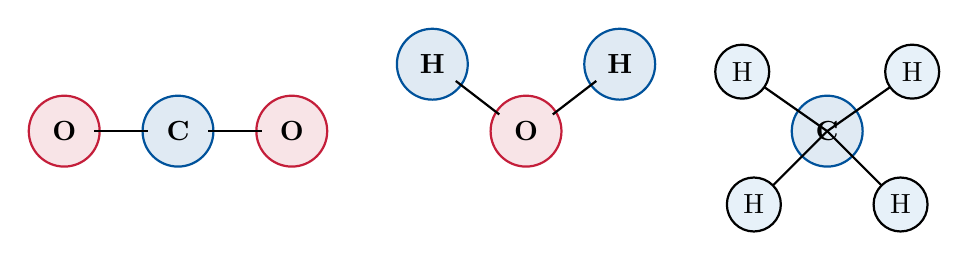
\begin{tikzpicture}[scale=.85,thick]
\atom{0,0}{C}{JapanBlue}\atom{-1.7,0}{O}{ChinaRed}\atom{1.7,0}{O}{ChinaRed}\draw (-1.25,0)--(-.45,0);\draw (.45,0)--(1.25,0);
\begin{scope}[xshift=5.2cm]\atom{0,0}{O}{ChinaRed}\atom{-1.4,1.0}{H}{JapanBlue}\atom{1.4,1.0}{H}{JapanBlue}\draw (-.4,.25)--(-1.05,.75);\draw (.4,.25)--(1.05,.75);\end{scope}
\begin{scope}[xshift=9.7cm]\atom{0,0}{C}{JapanBlue}\foreach \a in {35,145,225,315}{\draw (0,0)--(\a:1.35);\node[circle,draw,fill=SoftBlue,minimum size=6mm] at (\a:1.55){H};}\end{scope}
\end{tikzpicture}
\end{frame}

\begin{frame}{例題7｜ルイス構造：問題}
\def\exq{次の分子のルイス構造を書き、単結合・二重結合・三重結合の数を答えよ。\quad (1) H$_2$O \quad (2) CO$_2$ \quad (3) N$_2$}
\only<1>{\vfill\questioncard{\exq}\vfill}
\only<2>{\questioncard{\exq}\vfill
\begin{center}\Large
(1) $\mathrm{H-O-H}$\quad (Oに孤电子对2対)\\[1.5ex]
(2) $\mathrm{O=C=O}$\qquad (3) $\mathrm{N\equiv N}$
\end{center}
\answercard{H$_2$O：单键2；CO$_2$：双键2；N$_2$：三键1。先核对总价电子数再判断多重键。}}
\end{frame}

\begin{frame}{例題8｜分子の極性：問題}
\def\exq{HCl、CO$_2$、H$_2$O、CH$_4$ を極性分子と無極性分子に分類せよ。結合の極性だけでなく分子の形も用いて説明せよ。}
\only<1>{\vfill\questioncard{\exq}\vfill}
\only<2>{\questioncard{\exq}\vfill
\reasonflow{键是否有极性}{确定分子几何结构}{偶极矢量是否抵消}
\answercard{極性分子：HCl、H$_2$O。無極性分子：CO$_2$、CH$_4$。后两者结构对称，键偶极抵消。}}
\end{frame}

% ================================================================
\section{分子間力と結晶}

\begin{frame}{分子内の結合と分子間力を区別する}
\centering
\begin{tikzpicture}[>=Latex]
\node[circle,draw=ChinaRed,fill=SoftRed,minimum size=10mm] (o1) at (-3,0){O};
\node[circle,draw=JapanBlue,fill=SoftBlue,minimum size=8mm] (h11) at (-4.1,.8){H};
\node[circle,draw=JapanBlue,fill=SoftBlue,minimum size=8mm] (h12) at (-1.9,.8){H};
\draw[very thick] (o1)--(h11);\draw[very thick] (o1)--(h12);
\node[circle,draw=ChinaRed,fill=SoftRed,minimum size=10mm] (o2) at (3,0){O};
\node[circle,draw=JapanBlue,fill=SoftBlue,minimum size=8mm] (h21) at (1.9,.8){H};
\node[circle,draw=JapanBlue,fill=SoftBlue,minimum size=8mm] (h22) at (4.1,.8){H};
\draw[very thick] (o2)--(h21);\draw[very thick] (o2)--(h22);
\draw[densely dashed,line width=2pt,Purple] (h12)--(o2) node[midway,below]{水素結合};
\node[JapanBlue] at (-3,-1.35){分子内：共有結合（强）};
\node[Purple] at (3,-1.35){分子間：分子間力（较弱）};
\end{tikzpicture}
\begin{alertblock}{相变时发生什么？}
水沸腾时主要克服\key{分子间力}，不会把H$_2$O分解成H和O。
\end{alertblock}
\end{frame}

\begin{frame}{三つの主要な分子間力}
\small
\centering
\begin{tabular}{p{29mm}p{52mm}p{35mm}}\toprule
種類 & 発生条件・原因 & 例\\\midrule
分散力 & 瞬时电子偏移产生的临时偶极；所有分子都有 & He、I$_2$、CH$_4$\\
双極子間力 & 极性分子间正负端取向吸引 & HCl、SO$_2$\\
水素結合 & H与F、O、N结合后，同另一分子的孤电子对强烈吸引 & HF、H$_2$O、NH$_3$\\\bottomrule
\end{tabular}
\vfill
\begin{block}{大致强弱}
相近大小的分子中：水素結合 $>$ 双極子間力 $>$ 分散力。
\end{block}
\begin{alertblock}{但要比较分子大小}
电子数多、极化性大的大分子可有很强的分散力，例如 I$_2$ 常温为固体。
\end{alertblock}
\end{frame}

\begin{frame}{沸点を決める二つの視点}
\begin{columns}[T,onlytextwidth]
\column{.48\textwidth}
\begin{block}{1　分子間力の種類}
水素結合存在时，沸点往往显著升高。
\[
\mathrm{H_2O>H_2S}
\]
\end{block}
\column{.48\textwidth}
\begin{exampleblock}{2　分子の大きさ・形}
同类型分子中，相对分子质量和接触面积越大，分散力一般越强。
\[
\mathrm{I_2>Br_2>Cl_2>F_2}
\]
\end{exampleblock}
\end{columns}
\vfill
\centering
\begin{tikzpicture}[x=1.15cm,y=.022cm,>=Latex]
\draw[->] (0,0)--(8.3,0) node[right]{物質};\draw[->] (0,0)--(0,125) node[above]{沸点/$^\circ$C};
\foreach \x/\h/\t/\c in {1/20/HF/JapanBlue,3/-60/HCl/ChinaRed,5/-85/HBr/ChemGreen,7/-35/HI/Gold}{
\draw[line width=8pt,\c] (\x,0)--(\x,{\h+90});\node[below] at (\x,0){\t};}
\node[align=left] at (4.2,105){HF因水素結合而异常高};
\end{tikzpicture}
\end{frame}

\begin{frame}{分子結晶（分子晶体）}
\begin{columns}[c,onlytextwidth]
\column{.50\textwidth}
\centering
\begin{tikzpicture}[scale=.72]
\foreach \x/\y in {0/0,2/0,4/0,1/1.7,3/1.7,5/1.7,0/3.4,2/3.4,4/3.4}{
\node[ellipse,draw=JapanBlue,fill=SoftBlue,minimum width=13mm,minimum height=7mm] at (\x,\y){$\mathrm{I_2}$};}
\foreach \a/\b/\c/\d in {0.7/0/1.3/0,2.7/0/3.3/0,1.7/1.7/2.3/1.7,3.7/1.7/4.3/1.7,.7/3.4/1.3/3.4}{\draw[dashed,Purple,thick] (\a,\b)--(\c,\d);}
\node[Purple] at (2.5,-.8){分子間力};
\end{tikzpicture}
\column{.46\textwidth}
\begin{block}{構成粒子}
独立的分子。分子内共价键强，但分子之间作用较弱。
\end{block}
\begin{itemize}
  \item 融点・沸点低いものが多い
  \item 軟らかい
  \item 基本不导电
  \item 例：冰、干冰、碘、萘
\end{itemize}
\end{columns}
\end{frame}

\begin{frame}{共有結合の結晶（共价晶体）}
\begin{columns}[c,onlytextwidth]
\column{.52\textwidth}
\centering
\begin{tikzpicture}[scale=.75,thick]
\foreach \x/\y in {0/0,2/0,4/0,1/1.6,3/1.6,5/1.6,0/3.2,2/3.2,4/3.2}{\fill[JapanBlue] (\x,\y) circle (4pt);}
\foreach \a/\b/\c/\d in {0/0/1/1.6,2/0/1/1.6,2/0/3/1.6,4/0/3/1.6,4/0/5/1.6,1/1.6/0/3.2,1/1.6/2/3.2,3/1.6/2/3.2,3/1.6/4/3.2,5/1.6/4/3.2}{\draw[JapanBlue] (\a,\b)--(\c,\d);}
\node at (2.5,-.7){整体由共有結合构成};
\end{tikzpicture}
\column{.44\textwidth}
\begin{block}{特点}
不存在独立分子，原子通过共价键无限连接成巨大网状结构。
\end{block}
\begin{itemize}
  \item 融点非常高
  \item 硬，不易溶解
  \item 多数不导电
  \item 例：ダイヤモンド、Si、SiO$_2$、SiC
\end{itemize}
\begin{alertblock}{例外}
黒鉛可导电且层间较软。
\end{alertblock}
\end{columns}
\end{frame}

\begin{frame}{ダイヤモンドと黒鉛：同じCでも違う}
\small
\begin{columns}[T,onlytextwidth]
\column{.48\textwidth}
\begin{block}{ダイヤモンド}
\begin{itemize}
  \item 各C与4个C成键
  \item 三维网状结构
  \item 极硬、绝缘体
\end{itemize}
\centering
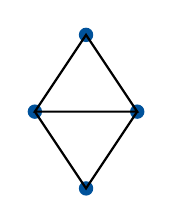
\begin{tikzpicture}[scale=.65,thick]
\foreach \x/\y in {0/0,2/0,1/1.5,1/-1.5}{\fill[JapanBlue] (\x,\y) circle (4pt);}
\draw (0,0)--(2,0)--(1,1.5)--cycle;\draw (0,0)--(1,-1.5)--(2,0);
\end{tikzpicture}
\end{block}
\column{.48\textwidth}
\begin{exampleblock}{黒鉛}
\begin{itemize}
  \item 各C与3个C成键
  \item 层内有可移动电子
  \item 可导电，层间易滑动
\end{itemize}
\centering
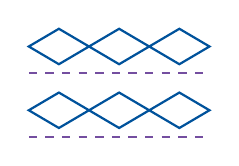
\begin{tikzpicture}[scale=.45,thick]
\foreach \y in {0,1.8}{\foreach \x in {0,1.7,3.4}{\draw[JapanBlue] (\x,\y) -- ++(.85,.5)--++(.85,-.5)--++(-.85,-.5)--cycle;}}
\draw[dashed,Purple] (0,-.75)--(5.1,-.75);\draw[dashed,Purple] (0,1.05)--(5.1,1.05);
\end{tikzpicture}
\end{exampleblock}
\end{columns}
\end{frame}

\begin{frame}{四種類の結晶を比較する}
\scriptsize
\centering
\begin{tabular}{p{20mm}p{23mm}p{26mm}p{26mm}p{28mm}}\toprule
結晶 & 構成粒子 & 粒子間の力 & 代表的性質 & 例\\\midrule
イオン結晶 & 陽・陰イオン & イオン結合 & 高融点、融解・水溶液で導電 & NaCl, MgO\\
分子結晶 & 分子 & 分子間力 & 低融点、軟、不導体 & I$_2$, CO$_2$, H$_2$O\\
共有結合の結晶 & 原子 & 共有結合 & 非常に高融点、硬 & C, Si, SiO$_2$\\
金属結晶 & 金属原子・自由電子 & 金属結合 & 導電、展性・延性 & Fe, Cu, Al\\\bottomrule
\end{tabular}
\vfill
\begin{alertblock}{判断顺序}
\centering 先判断构成粒子，再判断粒子间作用；不要只凭“是否含金属元素”机械判断复杂物质。
\end{alertblock}
\end{frame}

\begin{frame}{例題9｜分子間力と沸点：問題}
\def\exq{CH$_4$、NH$_3$、H$_2$O の沸点を高い順に並べよ。分子間力と分子構造を用いて説明せよ。}
\only<1>{\vfill\questioncard{\exq}\vfill}
\only<2>{\questioncard{\exq}\vfill
\reasonflow{CH$_4$は分散力のみ}{NH$_3$とH$_2$Oは水素結合}{H$_2$Oは強い網目を形成}
\answercard{$\boxed{\mathrm{H_2O>NH_3>CH_4}}$。H$_2$O每个分子能形成更发达的氢键网络；CH$_4$无极性，只有分散力。}}
\end{frame}

\begin{frame}{例題10｜結晶の分類：問題}
\def\exq{NaCl、ドライアイス、ダイヤモンド、銅を、イオン結晶・分子結晶・共有結合の結晶・金属結晶に分類し、常温固体で電気を通すものを選べ。}
\only<1>{\vfill\questioncard{\exq}\vfill}
\only<2>{\questioncard{\exq}\vfill
\begin{center}\begin{tabular}{c c}\toprule 物質 & 分類\\\midrule NaCl & イオン結晶\\ ドライアイス & 分子結晶\\ ダイヤモンド & 共有結合の結晶\\ 銅 & 金属結晶\\\bottomrule\end{tabular}\end{center}
\answercard{常温固体で导电的是\jp{銅}。NaCl固体中离子不能移动；金属中自由电子可移动。}}
\end{frame}

\begin{frame}{例題11｜性質から物質を見抜く：問題}
\def\exq{未知固体Aは高融点で、固体では電気を通さないが融解すると通す。Bは非常に硬く高融点で、固体・融解状態とも基本的に不導体である。A、Bの結晶の種類を答えよ。}
\only<1>{\vfill\questioncard{\exq}\vfill}
\only<2>{\questioncard{\exq}\vfill
\reasonflow{导电条件}{构成粒子是否移动}{结合方式を特定}
\answercard{A：\jp{イオン結晶}。B：\jp{共有結合の結晶}。A在融解时离子可移动；B无自由带电粒子。}}
\end{frame}

% ================================================================
\section{総合練習}

\begin{frame}{総合練習1｜問題}
\small
\begin{enumerate}
  \item 原子番号16の元素について、殻表示・周期・族・価電子数・安定な単原子イオンを答えよ。
  \item O$^{2-}$、F$^-$、Na$^+$、Mg$^{2+}$ はすべて電子数10である。半径を大きい順に並べよ。
  \item Mg と N からできるイオン結晶の組成式を書け。
  \item CO$_2$ と H$_2$O のうち極性分子を選び、理由を答えよ。
  \item SiO$_2$ と CO$_2$ はともに酸化物だが融点が大きく異なる。結晶構造から説明せよ。
\end{enumerate}
\vfill
\centering\key{先不要翻答案：每题先写出“判断依据”。}
\end{frame}

\begin{frame}{総合練習1｜解答}
\small
\begin{enumerate}
  \item $2,8,6$；第3周期、16族、价电子6、$\mathrm{S^{2-}}$。
  \item 等电子体中核电荷越大半径越小：$\mathrm{O^{2-}>F^->Na^+>Mg^{2+}}$。
  \item $\mathrm{Mg^{2+}}$ 与 $\mathrm{N^{3-}}$ 电荷平衡：$\boxed{\mathrm{Mg_3N_2}}$。
  \item H$_2$O为极性分子；折线形使键偶极不抵消。CO$_2$直线对称，抵消。
  \item SiO$_2$是共有結合の結晶，需破坏大量共价键；CO$_2$是分子結晶，熔化仅需克服较弱分子间力。
\end{enumerate}
\end{frame}

\begin{frame}{総合練習2｜EJU形式・問題}
\small
元素X、Y、Z的最外层电子数分别为1、7、8，且三者均位于第3周期。回答：
\begin{enumerate}
  \item 写出X、Y、Z的元素符号。
  \item 比较X与Y的原子半径。
  \item 写出X与Y形成化合物的组成式和结合类型。
  \item 说明该化合物在固体和水溶液中导电性的差异。
  \item 三者中第一イオン化エネルギー最大的是谁？
\end{enumerate}
\end{frame}

\begin{frame}{総合練習2｜解答}
\small
\begin{enumerate}
  \item 第3周期：X=Na、Y=Cl、Z=Ar。
  \item 同周期向右原子半径减小，所以 $\mathrm{Na>Cl}$。
  \item $\mathrm{NaCl}$，イオン結合。
  \item 固体中离子位置固定，不导电；水溶液中 $\mathrm{Na^+}$、$\mathrm{Cl^-}$ 可移动，导电。
  \item Ar。闭壳层结构稳定，移走电子最困难。
\end{enumerate}
\begin{alertblock}{一题贯通}
\centering 周期表位置 $\rightarrow$ 原子性质 $\rightarrow$ 电子授受 $\rightarrow$ 结合与宏观性质
\end{alertblock}
\end{frame}

\begin{frame}{重要語彙}
\small
\begin{multicols}{2}
\begin{itemize}
  \item 電子配置（でんしはいち）
  \item 電子殻（でんしかく）
  \item 最外殻電子（さいがいかくでんし）
  \item 価電子（かでんし）
  \item 周期律（しゅうきりつ）
  \item 周期表（しゅうきひょう）
  \item 族（ぞく）・周期（しゅうき）
  \item 原子半径（げんしはんけい）
  \item イオン化エネルギー
  \item 電気陰性度（でんきいんせいど）
  \item イオン結合（けつごう）
  \item イオン結晶（けっしょう）
  \item 共有結合（きょうゆうけつごう）
  \item 共有電子対（きょうゆうでんしつい）
  \item 非共有電子対（ひきょうゆうでんしつい）
  \item 分子間力（ぶんしかんりょく）
  \item 水素結合（すいそけつごう）
  \item 分子結晶（ぶんしけっしょう）
  \item 共有結合の結晶
\end{itemize}
\end{multicols}
\end{frame}

\begin{frame}{まとめ：判断のチェックリスト}
\begin{columns}[T,onlytextwidth]
\column{.48\textwidth}
\begin{block}{原子・周期表}
\begin{enumerate}
  \item 原子番号から電子数
  \item 電子配置から周期・族
  \item 価電子から离子与结合倾向
  \item 周期趋势比较半径和能量
\end{enumerate}
\end{block}
\column{.48\textwidth}
\begin{exampleblock}{結合・結晶}
\begin{enumerate}
  \item 電子授受还是電子共有？
  \item 構成粒子是什么？
  \item 粒子间作用是什么？
  \item 带电粒子能移动吗？
\end{enumerate}
\end{exampleblock}
\end{columns}
\begin{alertblock}{最后一句}
\centering \jp{微观结构决定宏观性质。}所有分类题都要写清“构成粒子”和“粒子间作用”。
\end{alertblock}
\end{frame}

\begin{frame}{宿題}
\small
\begin{enumerate}
  \item P、K、Ca 的電子配置、周期、族、価電子数を求める。
  \item $\mathrm{Al^{3+}}$、$\mathrm{O^{2-}}$、$\mathrm{F^-}$ の電子数と半径を比較する。
  \item $\mathrm{Ca^{2+}}$ と $\mathrm{PO_4^{3-}}$ から組成式を作る。
  \item NH$_3$、H$_2$O、CO$_2$、CH$_4$ のルイス構造と分子の極性を判定する。
  \item HF、HCl、HBr、HI 的沸点差异を説明する。
  \item NaCl、I$_2$、SiO$_2$、Cu 的结晶类型、熔点特点及导电性を表にまとめる。
  \item “固体不导电、熔融导电”这一现象为什么能作为离子晶体的线索？用三句话回答。
\end{enumerate}
\vfill
\centering\jp{答えだけでなく、電子配置・構造・力の三段階を書こう。}
\end{frame}

\end{document}
